\documentclass[times]{sig-alternate}
\usepackage{epsfig}
\usepackage{subfigure}


\textwidth 16.0cm \textheight 23.0cm
\oddsidemargin -0.1in
\evensidemargin -0.1in
\topmargin -0.5in
\parskip 0.25ex
\parindent 1.5ex
\sloppy
\raggedbottom


\def \ie {{\it i.e.}, }
\def \eg {{\it e.g.}, }

\newcommand{\tile}{tile}
\newcommand{\Tile}{Tile}
\newcommand{\tiles}{tiles}
\newcommand{\Tiles}{Tiles}
\newcommand{\ntiles}{16}

\newlength{\itemhack}
\setlength{\itemhack}{-0.088in}

\newlength{\parhack}
\setlength{\parhack}{-0.12in}


\begin{document}


%\section{Introduction}
As more and more parts of modern life use digital computation, everything from cell phones, GPS systems
and satellite radios, require ever more complicated processing of digital signals. 
Each successive generation of applications requires ever more sophisticated algorithms mapped 
on to ever more specialized digital signal processors (DSP). As 
embedded devices have severe performance requirements placed on them,
the mapping of algorithm to architecture is typically done by hand at great cost and great expense.

Upward of fifty percent of the code that runs the DSP(s) in a modern cell phone is coded in assembly
with the rest written in C. Hand optimized assembly code typically makes the best use of the 
available resources such as power, specialized coprocessors, and specialized instructions.
The problem with assembly code is that the same algorithm must be mapped time and time again 
whenever a new chip comes out. The life cycle of a typical DSP is much shorter than the life
cycle of a general purpose microprocessor -- each new generation is separated by months rather
than years.
 
Therefore frequently reimplementing algorithms by hand is a costly arduous process that 
increases cost and slows the pace of advances. Engineers must spend time working out details rather 
than focusing on solving harder problems. Compilers were invented forty years ago 
exactly to let engineers focus on the problem at hand rather than spend time with 
machine specific details. Compilers for DSP architectures have a difficult job, and are not
very good at mapping a program written in a general purpose language like C into the specialized 
instructions provided by DSPs. Many of the instructions provided by a DSP are targeted 
for a very specific application (like FIR filtering), but most general purpose languages have
no way to describe higher level behavior other than functionally. If you don't express
your algorithm in the same way that the compiler expects to encounter it, the resulting
program will not take best advantage of the available DSP resources.

We are attempting to solve this problem by introducing a new domain specific language which
supports imperative C like code to describe computation. By imposing structure and
explicitly identifying the input and the output of different program sub components
we can run an analysis that determine if a program is performing a common DSP task.  
We can then use this information to take advantage of special purpose DSP hardware
or we can even apply standard signal processing algorithm optimizations to 
We can then leverage the existing work on DSP algorithm optimization to perform compiler transformation
at a fairly sophisticated level. Our system lets programmers describe the
computation to be performed at an appropriate level and the compiler takes care of 

\subsection{Motivating Example}
\begin{figure}
\center
\epsfxsize=2.0in
\epsfbox{images/motivating-example.eps}

\begin{verbatim}
float data[N]; /* input data buffer */
float buffer[N]; /* inter-filter buffer */

/* initialize inter-filter buffer */
for (i=0; i<N; i++) {
  /* filter starting at index i of input data, wrap around */
  buffer[i] = filter(weights1, data, i, N);
  data[i] = get_next_input();
}

i = 0;
while(true) {
  push_output(filter(weights2, buffer, i, N));
  /* get next data item */
  data[i] = get_next_input();
  /* generate the next element in the inter filter buffer */
  buffer[i] = filter(weights1, data, i, N);
  /* update current start of buffer */
  i = (i+1)%N
}
\end{verbatim}
\caption{FIR filtering with back to back filters in C. Note the use of circular buffers.}
\label{fig:motivating-example}
\end{figure}

As an example of the types of program transformation that our optimization allows,
consider a sequence of finite impulse response (FIR) filters as shown in 
Figure~\ref{fig:motivating-example}. The imperative C style code that implements
this simple DSP application is also shown. The program largely defies many
standard compiler analysis and optimization techniques because of its use of circular
buffers and the muddled relationship between {\tt data}, {\tt buffer} and the output.

\begin{figure}
\begin{verbatim}
float->float pipeline TwoPipe {
  add FIRFilter(weights1);
  add FIRFilter(weights2);
}

float->float filter FIRFilter(float[N] weights) {
  work push 1 pop 1 peek N {
    float sum = 0;
    for (int i=0; i<N; i++) {
      sum += weights[i] * peek(i);
    }
    push(sum);
    pop();
}
\end{verbatim}
\caption{StreamIt program to implement the same processing as the program in Figure~\ref{fig:motivating-example}}
\label{fig:example-streamit}
\end{figure}


Figure~\ref{fig:example-streamit} shows the same filtering process implemented in 
StreamIt. The StreamIt program is better because it uses explicit input/output channels,
lets the compiler worry about buffer management and shows the structure of the original
block diagram. 


\begin{figure}
\begin{verbatim}
float->float filter LinearTwoPipe() {
  work push 1 pop 1 peek N {
    float sum = 0;
    for (int i=0; i<N; i++) {
      sum += combined_weights[i]*peek(i);
      }
    push(sum);
    pop();
  }
}
\end{verbatim}
\caption{Program after combination in psuedo-StreamIt.}
\label{fig:example-combine}
\end{figure}

Our data analysis provides a complete relationship between input and output for
each filter, and furthermore can combine the actions of the two filters as shown
in Figure~\ref{fig:example-combine}. The new combined filter's {\tt combined\_weights}
array contains elements such that the overall output is the same.

\begin{figure}
\begin{verbatim}
float->float filter FreqTwoPipe() {
  complex[N] H;
  init {
    H = FFT(combined_weights);
  }
  work push L pop L peek N+L {
    float[N] X = FFT(peek(0..N+L-1)); /* input FFT */
    float[N] Y =  X .* H; /* element wise mult */
    float[N] y = IFFT(Y); /* inverse FFT */
    push(y[0..L-1]); /* push first L elts of y */
  }
}
\end{verbatim}
\caption{Program after using the FFT to implement the filter in psuedo-StreamIt.}
\label{fig:example-frequency}
\end{figure}

Out compiler can actually go one step farther and apply a well known 
optimization to calculate the output values using a frequency transformation
as is outlined in psuedo code in Figure~\ref{fig:example-frequency}.




\subsection{StreamIt}

\begin{figure}
\center
\epsfxsize=3.0in
\epsfbox{images/general-picture-filter.eps}
\caption{Graphical illustration of $e_{F}$, $o_{F}$ and $u_{F}$}
\label{fig:overview-filter}
\end{figure}


The StreamIt\cite{streamitcc, streamit-asplos, gordon-thesis} language
aims to provide a language and compiler for streaming applications. Streaming applications 
are characterized by data streaming in and out of the application. Each data element (both
input and output) is in the system for only a small amount of time as opposed to scientific
applications where the data set is typically used extensively over the execution time.

StreamIt programs are composed of processing blocks called {\tt filters} which
contain an input tape from which they can read values and an output tape to which
they can write. Each {\tt filter} contains a {\tt work} function which describes 
a steady state computation that consumes input and produces output.
{\tt filters } can examine data items  on the input tape without consuming them 
via {\tt peek} expressions. {\tt pop} expressions consume data from the input
tape. A {\tt filter} calls {\tt push} to add values to the output tape.
{\tt filters} can contain stateful fields that persist between calls to {\tt work}. 
The {\tt work} function is C-like imperative code, 
which can access {\tt filter} state, call external routines and produce and consume data. 
There are few restrictions on a {\tt work} function other than the requirement that
it consume input and produce output at the stated rates.

All {\tt filters} in StreamIt declare the number of elements they
will {\tt peek} at, the number of elements they will {\tt pop} and the number
of elements that they will {\tt push}. A {\tt Filter} $F$ can examine up to $e_F$ 
items from its input tape, consumes exactly $o_F$ items and produces exactly
$u_F$ items. Currently StreamIt requires that each filter has declared $e_F$, $o_F$ 
and $u_F$ that are statically determinable at compile time. 
Figure~\ref{fig:overview-filter} shows how $e_F$, $o_F$ and $u_F$ are related.

\begin{figure}
\center
\epsfxsize=3.0in
\epsfbox{images/streamit-structures.eps}
\caption{StreamIt structures: {\tt pipeline}, {\tt splitjoin}, and {\tt feedbackloop}.}
\label{fig:structures}
\end{figure}

{\tt filters} in StreamIt are composed hierarchically using predefined structures to form
a program. 

\begin{enumerate}
\item {\tt pipelines} represent the serial computation of one filter after another.
\item {\tt splitjoins} represent explicitly parallel computation. 
\item {\tt feedbackloops} allow cycles to be introduced into the stream graph. 
\end{enumerate}

{\tt filters}, {\tt pipelines}, {\tt splitjoins} and {\tt feedbackloops} 
are all {\tt streams} and each {\tt stream} can be used as a subcomponent in 
a structure. Figure~\ref{fig:structures} illustrates the three structures 
provided as primitives in StreamIt.
StreamIt programs can therefore be represented as a connected graph of filters 
which we will refer to as the stream graph. It is also important to note
{\tt streams} have exactly one input tape and one exactly one output tape.

Most real world programs can be fit into StreamIt's structured stream model, 
though the fit sometimes requires extra manipulation. We believe
that benefits of structure to both the programmer and the compiler outweigh the
costs of imposing structure on the programmer.

\subsection{Matrices and DSP}
We take advantage of StreamIt's explicit input and output tapes and
our knowledge that a large class of StreamIt programs will be performing
standard digital signal processing (DSP) operations to generate useful
optimizations.

There is an entire research area in Electrical Engineering devoted to DSP. The
theory and the implementation of systems to process digital signals is well developed (see
an introductory text such as\cite{oppenheim-discrete} or \cite{lyons-understanding}). 
There are a few fundamental primitives used to describe most DSP systems, and the output of 
most of these primitives can be expressed as a linear combination of their inputs. Examples are
finite impulse response (FIR) filters, compressors, expanders and signal processing transforms
such as the discrete Fourier transform (DFT) and discrete cosine transformation (DCT).

Electrical engineers who concentrate on DSP applications spend a large percentage of their 
time designing an appropriate implementation given a particular design. Choosing
the appropriate implementation structure is a highly non trivial task, and sometimes determining the 
the ``right'' choice is often more of an art than a science. There are many systems that allow a
designer to explore design choices such as Matlab\cite{matlab} which is used extensively in
both academia and industry.  There are also research projects such as \cite{covell-ade} 
and those described in \cite{oppenheim-symbolic} aimed at allowing a DSP designer to explore
various implementation choices.(XXXXXXXXXXXXx -- Are there other things we should reference here?) 

Given that a product called Matlab (as in  MATrix LAB) is used extensively
in DSP applications, it is probably not surprising that matrices often provide 
a convenient way of working with digital data and for describing digital filters. 
If a {\tt work} function is doing matrix computation, by recognizing this fact
we can take advantage of the huge body of existing knowledge.

\Section{StreamIt Programming Language}
\label{sec:streamit}

StreamIt~\cite{streamit-cc} is an architecture independent language
that is designed for stream programming. In StreamIt, programs are
represented as graphs where nodes represent computation and edges
represent FIFO-ordered communication of data over tapes. The language
features several novelties that are essential for large scale program
development. The language is modular, parameterizable, malleable and
architecture independent. In addition, the language exposes the
inherent parallelism and communication patterns that are prevalent in
streaming programs.

\begin{figure*}[t]
  \begin{minipage}[t]{4.0in}
    {
	\begin{scriptsize}
	  \begin{verbatim}
	    int->int filter ZigZagScan(int N, int[N] Order)
	    {
	        work pop N push N {
	        for (int i = 0; i < N; i++) {
	          int pixel = peek(Order[i]);
	          push(pixel);
	        }
	        for (int i = 0; i < N; i++) {
	          pop();
	        }
	      }
	    }
	  \end{verbatim}
	\end{scriptsize}
    }
    % \vspace{-3pt}
    \caption{Example filter implementing zig-zag scanning.}
    % \label{fig:zigzag-filter}
  \end{minipage}
  ~~\vrule~~
  \begin{minipage}[t]{3.0in}
    {  
	\begin{scriptsize}
	  \begin{verbatim}
	    int[64] Ordering = 
	      {00, 01, 05, 06, 14, 15, 27, 28,
	       02, 04, 07, 13, 16, 26, 29, 42,
	       03, 08, 12, 17, 25, 30, 41, 43,
	       09, 11, 18, 24, 31, 40, 44, 53,
	       10, 19, 23, 32, 39, 45, 52, 54,
	       20, 22, 33, 38, 46, 51, 55, 60,
	       21, 34, 37, 47, 50, 56, 59, 61,
	       35, 36, 48, 49, 57, 58, 62, 63};



	  \end{verbatim}
	\end{scriptsize}
    }
    % \vspace{-3pt}
    \caption{Example zig-zag order for filter.}
    \label{fig:zigzag-order}
  \end{minipage}
\end{figure*}

\SubSection{Filters as Programmable Units}
In StreamIt, the basic programmable unit is a {\it filter}. Each
filter contains a work function that executes atomically, popping
(i.e., reading) a fixed number of items from the filter input tape
and pushing (i.e., writing) a fixed number of items to the filter
output tape. A filter may also {\tt peek} at a given index on its
input tape without consuming the item; this makes it simple to
represent computation over a sliding window or performing permutations
on the input stream. The {\tt push}, {\tt pop}, and {\tt peek} rates
are declared as part of the work function, thereby enabling the
compiler to apply various optimizations and construct efficient
execution schedules. 

A filter is akin to a class in object oriented programming with the
work function serving as the main method. A filter is parameterizable,
and this allows for greater malleability and code reuse. An example
filter is shown in Figure~\ref{fig:zigzag-filter}. This filter
consumes a stream whose elements are of type {\tt int} and produces a
stream of the same type. It implements the zig-zag scanning pattern
used in the run-length encoding of quantized DCT coefficients (see
Figure~\ref{fig:zigzag}). Typically, the zig-zag scan operates on a
8x8 matrix. An instantiation of a filter can specify the matrix
dimensions, as well as the desired ordering. In MPEG, there are two
possible scan orders. The {\tt Order} parameter can define the
specific scan pattern that is desired. For example, to implement the
order shown in Figure~\ref{fig:zigzag}(a), the array is defined as
shown in Figure~\ref{fig:zigzag-order}.

In this example, the DCT matrix is represented as a unidimensional
stream. The filter peeks or inspects the elements and copies them to
the output stream in the specified order. Once all the DCT
coefficients are copies, the input stream is deallocated from the tape
with a series of pops.

\begin{figure}[t]
\begin{center}
%\vspace{-24pt}
% \framebox{
 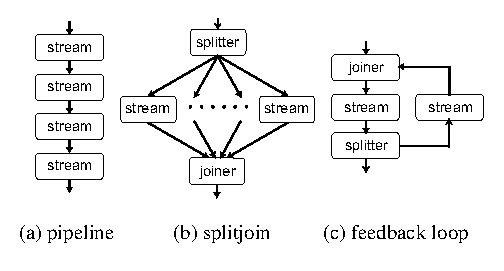
\includegraphics[scale=1, angle=0]{./constructs-eg.eps}
%}
% \vspace{-6pt}
% \nocaptionrule
 \caption{Hierarchical streams in StreamIt.}
 \label{fig:containers}
\end{center}
\end{figure}

\SubSection{Hierarchical Streams}
In StreamIt, the application developer focuses on the hierarchical
assembly of the stream graph and its communication topology, rather
than on the  explicit management of the data buffers between filters.
StreamIt provides three hierarchical structures for composing filters
into larger stream graphs (see Figure~\ref{fig:containers}).

\paragraph{Pipeline.}
The {\it pipeline} stream construct composes streams in sequence, with
the output of one connected to the input of the next.  An example of a
pipeline appears in Figure~\ref{fig:decoder-pipeline}. A pipeline is a
single input to single output stream. The decoding pipeline in the
figure consists of three streams. The first is a filter which zig-zag
unorders the input stream, and prepares the data for the inverse
quantization and DCT. The output of the filter is consumed by a stream
named {\tt IQ} which is a pipeline itself (not shown). This example
illustrates the hierarchical nature of stream composition in
StreamIt. The {\tt IQ} pipeline performs the inverse quantization, and
produces an output stream that is in turn consumed by another stream
which performs the inverse DCT. As in the case of a filter, pipelines
are also parameterizable.

\begin{figure*}[t]
  \begin{scriptsize}
    \begin{verbatim}
	int->int pipeline Decode()
	{ 
	  int Order[64] = {...};     // initialized as shown earlier
	  add ZigZagScan(64, Order);
	  add IQ();                  // inverse quantization
	  add IDCT(8, 8);            // inverse DCT (8x8 matrix)
	}
    \end{verbatim}
  \end{scriptsize}
  % \vspace{-3pt}
  \caption{Example MPEG decoder pipeline.}
  \label{fig:decoder-pipeline}
\end{figure*}

The {\tt add} keyword in StreamIt constructs the specified stream
using the input parameters. The {\tt add} statement may only appear in
non-filter streams.  In essence, filters are the leaves in the
hierarchical construction, and composite nodes in the stream graph
define the encapsulating containers. This allows for modular design
and development of large applications, thereby  promoting
collaboration, increasing code reuse, and simplifying debugging.

\paragraph{Split-Join.}
The {\it splitjoin} stream construct distributes data to a set of
parallel streams, which are then joined together in a roundrobin
fashion. In a splitjoin, the {\it splitter} performs the data
scattering, and the {\it joiner} performs the gathering. A splitter is
a specialized filter with a single input and multiple output
channels. On  every execution step, it can distribute its output to
any one of its children in either a {\it duplicate} or a {\it
roundrobin} manner. For the former, incoming data are replicated to
every sibling connected to the splitter. For the latter, data are
scattered in a roundrobin manner, with each item sent to exactly one
child stream, in order. The splitter type and the weights for
distributing data to child streams are declared as part of the syntax
(e.g., \texttt{split duplicate} or \texttt{split
roundrobin($w_1,\ldots,w_n$)}). The splitter counterpart is the
joiner. It is a specialized filter with  multiple input channels but
only one output channel. The joiner gathers data from its predecessors
in a roundrobin manner (declared as part of the syntax) to produce a
single output stream.

\begin{figure*}[t]
  \begin{scriptsize}
    \begin{verbatim}
	// N = macroblock size + motion vector data size;
	// W = picture width (resolution in pixels);
	// H = picture width (resolution in pixels);

	int->int splitjoin YCrCbDecoding(int N, int W, int H)
	{
	  // 4:2:0 chroma format
	  split roundrobin(4*N, 1*N, 1*N);

	  add LuminanceChannel  (W, H);
	  add ChrominanceChannel(W, H);
	  add ChrominanceChannel(W, H);

	  join roundrobin(1, 1, 1);  
	}
    \end{verbatim}
  \end{scriptsize}
  % \vspace{-3pt}
  \caption{Example MPEG decoder splitjoin.}
  \label{fig:decoder-sj}
\end{figure*}

The splitjoin stream is a convenient and natural way to represent
parallel computation. For example, when the decoder performs the
luminance and chrominance channel processing, the computation can
occur in parallel. In StreamIt, this is expressed as shown in
Figure~\ref{fig:decoder-sj}. The input stream contains the
macroblock data along with the parsed motion vectors. The data is
partitioned and passed to one of three decoding channels, with $4N$
items assigned to the first stream, $N$ items to the second, and $N$
items to the third. The three streams reconstruct the original
pictures with respect to the different color channels, and their
output is combined by the joiner to produce the final decoded picture.

\paragraph{Feedback Loop.}
StreamIt also provides a {\it feedback loop} construct for introducing
cycles in the graph. This stream construct is not used in the decoder,
but may be used in the MPEG encoder.

\paragraph{XXX: need to introduce messaging and talk about it.}
\input{rawbackend-phases}
\newcommand{\mt}[1]{\mbox{\it #1}}

\subsection{Stream Graph Partitioning}
\label{sec:partition}

StreamIt provides the filter construct as the basic abstract unit of
autonomous stream computation.  The programmer should decide the
boundaries of each filter according to what is most natural for the
algorithm under consideration.  While one could envision each filter
running on a separate machine in a parallel system, StreamIt hides the
granularity of the target machine from the programmer.  Thus, it is
the responsibility of the compiler to adapt the granularity of the
stream graph for efficient execution on a particular architecture.

We use the word {\it partitioning} to refer to the process of dividing
a stream program into a set of balanced computation units.  Given that
a maximum of $N$ computation units can be supported, the partitioning
stage transforms a stream graph into a set of no more than $N$
filters, each of which performs approximately the same amount of work
during the execution of the program.  Following this stage, each
filter can be run on a separate processor to obtain a load-balanced
executable.


\begin{figure}[!h]
  \psfig{figure=beam-blood-key.eps,width=3.0in} \\
  \subfigure[
    {\bf Original (runs on 64 tiles).}\label{fig:beam-blood1}]{\psfig{figure=beam-blood-orig.eps,width=3.1in}}
  \hspace{0.3in} \subfigure[
    {\bf Partitioned (runs on 16 tiles).}\label{fig:beam-blood2}]{\psfig{figure=beam-blood-opt.eps,width=3.1in}
    } \caption{\protect\small Execution
    traces for the (a) original and (b) partitioned versions of the
    Radar application.  The $x$ axis denotes time, and the $y$ axis
    denotes the processor.  Dark bands indicate periods where
    processors are blocked waiting to receive an input or send an
    output; light regions indicate periods of useful work.  The thin
    stripes in the light regions represent pipeline stalls.  Our
    partitioning algorithm decreases the granularity of the graph from
    53 unbalanced tiles (original) to 15 balanced tiles (partitioned).
    The throughput of the partitioned graph is 2.3 times higher than
    the original. \protect\label{fig:beam-blood}}
\end{figure}

Our partitioner employs a set of fusion, fission, and reordering
transformations to incrementally adjust the stream graph to the
desired granularity.  To achieve load balancing, the compiler
estimates the number of instructions that are executed by each filter
in one steady-state cycle of the entire program; then, computationally
intensive filters can be split, and less demanding filters can be
fused.  Currently, a simple greedy algorithm is used to automatically
select the targets of fusion and fission, based on the estimate of the
work in each node.

%\begin{figure}[htpb]
\begin{figure}[!h]
%\vspace{-.5in}
\centering
\begin{minipage}{3.0in}
\centering
\psfig{figure=beam-graph-orig.eps,width=2.5in}
\caption{\protect\small Stream graph of the original 12x4 Radar
application.  The 12x4 Radar application has 12 channels and 4 beams;
it is the largest version that fits onto 64 tiles without filter
fusion.  \protect\label{fig:beam-orig}}
\end{minipage}
\hspace{0.1in}
\begin{minipage}{3.0in}
\centering
\psfig{figure=beam-graph-opt.eps,width=1.9in}
\caption{\protect\small Stream graph of the load-balanced 12x4
Radar application.  Vertical fusion is applied to collapse each pipeline
into a single filter, and horizontal fusion is used to transform the
4-way splitjoin into a 2-way splitjoin.  Figure~\ref{fig:beam-blood}
shows the benefit of these
transformations. \protect\label{fig:beam-opt}}
\end{minipage}
\end{figure}


For example, in the case of the Radar application, the original
stream graph (Figure~\ref{fig:beam-orig}) contains 52 filters.  These
filters have unbalanced amounts of computation, as evidenced by the
execution trace in Figure~\ref{fig:beam-blood1}.  The partitioner
fuses all of the pipelines in the graph, and then fuses the bottom
4-way splitjoin into a 2-way splitjoin, yielding the stream graph in
Figure~\ref{fig:beam-opt}.  As illustrated by the execution trace in
Figure~\ref{fig:beam-blood2}, the partitioned graph has much better
load balancing.  In the following sections, we describe in more detail
the transformations utilized by the partitioner.


\subsubsection{Fusion Transformations}

Filter fusion is a transformation whereby several adjacent filters are
combined into one.  Fusion can be applied to decrease the granularity
of a stream graph so that an application will fit on a given target,
or to improve load balancing by merging small filters so that there is
space for larger filters to be split.  Analogous to loop fusion in the
scientific domain, filter fusion can enable other optimizations by
merging the control flow graphs of adjacent nodes, thereby shortening
the live ranges of variables and allowing independent instructions to
be reordered.



\subsubsection{Fission Transformations}

Filter fission is the analog of parallelization in the streaming
domain.  It can be applied to increase the granularity of a stream
graph to utilize unused processor resources, or to break up a
computationally intensive node for improved load balancing.


\subsubsection{Reordering Transformations}

There are a multitude of ways to reorder the elements of a stream
graph so as to facilitate fission and fusion transformations.  For
instance, neighboring splitters and joiners with matching weights can
be eliminated a splitjoin construct can be divided into a hierarchical
set of splitjoins to enable a finer granularity of fusion and
identical stateless filters can be pushed through a splitter or joiner
node if the weights are adjusted accordingly.

\subsubsection{Automatic Partitioning}

In order to drive the partitioning process, we have implemented a
simple greedy algorithm that performs well on most applications.  The
algorithm analyzes the {\tt work} function of each filter and
estimates the number of cycles required to execute it.  
In the case where there are fewer filters than tiles, the partitioner
considers the filters in decreasing order of their computational
requirements and attempts to split them using the filter fission
algorithm described above.  
If the stream graph contains more nodes than the target architecture,
then the partitioner works in the opposite direction and repeatedly
fuses the least demanding stream construct until the graph will fit on
the target.  

Despite its simplicity, this greedy strategy works well in practice
because most applications have many more filters than can fit on the
target architecture; since there is a long sequence of fusion
operations, it is easy to compensate from a short-sighted greedy
decision.  However, we can construct cases in which a greedy strategy
will fail.  For instance, graphs with wildly unbalanced filters will
require fission of some components and fusion of others; also, some
graphs have complex symmetries where fusion or fission will not be
beneficial unless applied uniformly to each component of the graph.
We are working on improved partitioning algorithms that take these
measures into account.


\subsection{Layout}
\label{sec:layout}

The goal of the layout phase is to assign nodes in the stream graph to
computation nodes in the target architecture while minimizing the
communication and synchronization present in the final layout.  The
layout assigns exactly one node in the stream graph to one computation
node in the target.  The layout phase assumes that the given stream
graph will fit onto the computation fabric of the target and that the
filters are load balanced.  These requirements are satisfied by the
partitioning phase described above.

The layout phase of the StreamIt compiler is implemented using
simulated annealing \cite{simanneal}.  We choose simulated annealing
for its combination of performance and flexibility.  To adapt the
layout phase for a given architecture, we supply the simulated
annealing algorithm with three architecture-specific parameters: a
cost function, a perturbation function, and the set of legal layouts.
To change the compiler to target one tiled architecture instead of
another, these parameters should require only minor modifications.

The cost function should accurately measure the added communication
and synchronization generated by mapping the stream graph to the
communication model of the target.  Due to the static qualities of
StreamIt, the compiler can provide the layout phase with exact
knowledge of the communication properties of the stream graph.  The
terms of the cost function can include the counts of how many items
travel over each channel during an execution of the steady state.
Furthermore, with knowledge of the routing algorithm, the cost
function can infer the intermediate hops for each channel.  For
architectures with non-uniform communication, the cost of certain hops
might be weighted more than others.  In general, the cost function can
be tailored to suit a given architecture.

Phase ordering between stream graph parttioning and layout can lead to
suboptimal results. We plan to develop a unified approach for
partitioning and layout in the future.

\subsection{Communication Scheduler}
\label{sec:communic}

With the nodes of the stream graph assigned to computation nodes of
the target, the next phase of the compiler must map the communication
explicit in the stream graph to the interconnect of the target.  This
is the task of the communication scheduler.  The communication
scheduler maps the infinite FIFO abstraction of the stream channels to
the limited resources of the target.  Its goal is to avoid deadlock
and starvation while utilizing the parallelism explicit in the stream
graph.

The exact implementation of the communication scheduler is tied to the
communication model of the target.  The simplest mapping would occur
for targets implementing an end-to-end, infinite FIFO abstraction, in
which the scheduler needs only to determine the sender and receiver of
each data item.  This information is easily calculated from the
weights of the splitters and joiners.  As the communication model
becomes more constrained, the communication scheduler becomes more
complex, requiring analysis of the stream graph. For targets
implementing a finite, blocking nearest-neighbor communication model,
the exact ordering of tile execution must be specified.

Due to the static nature of StreamIt, the compiler can statically
orchestrate the communication resources.  As described in
Section~\ref{sec:phases}, we create an initialization schedule and a
steady-state schedule that fully describe the execution of the stream
graph.  The schedules can give us an order for execution of the graph
if necessary.  One can generate orderings to minimize buffer length,
maximize parallelism, or minimize latency.

Deadlock must be carefully avoided in the communication
scheduler. Each architecture requires a different deadlock avoidance
mechanism and we will not go into a detailed explanation of deadlock
here.  In general, deadlock occurs when there is a circular dependence
on resources.  A circular dependence can surface in the stream graph
or in the routing pattern of the layout.  If the architecture does not
provide sufficient buffering, the scheduler must serialize all
potentially deadlocking dependencies.


\subsection{Preliminary Results}
\label{sec:results}

\begin{table*}[!t]
\begin{center}
\scriptsize
\begin{tabular}{|l|l||r||r|r|r|r||r||} \hline
 & & {\bf lines of} & \multicolumn{4}{|c||}{\bf \# of constructs in the program} & {\bf \# of filters in the} \\ \cline{4-7}
{\bf Benchmark} & {\bf Description} & {\bf code} & filters & pipelines & splitjoins & feedbackloops & {\bf expanded graph}
\\
\hline \hline
FIR & 64 tap FIR & 
125 & 5 & 1 & 0 & 0 & 132
\\ \hline
Radar & Radar array front-end~\cite{pca} & 
549 & 8 & 3 & 6 & 0 & 52
\\ \hline
Radio & FM Radio with an equalizer & 
525& 14 & 6 & 4 & 0 & 26
\\ \hline
Sort & 32 element Bitonic Sort & 
419 & 4 & 5 & 6 & 0 & 242
\\  \hline
FFT & 64 element FFT & 
200 & 3 & 3 & 2 & 0 & 24
\\  \hline
Filterbank & 8 channel Filterbank & 
650 & 9 & 3 & 1 & 1 & 51
\\  \hline
GSM & GSM Decoder & 
2261 & 26 & 11 & 7 & 2 & 46
\\ \hline
Vocoder & 28 channel Vocoder~\cite{seneff80} &  
1964 & 55 & 8 & 12 & 1 & 101
\\ \hline
3GPP & 3GPP Radio Access Protocol~\cite{3gpp} &  
1087 & 16 & 10 & 18 & 0 & 48
\\ \hline
\hline
\end{tabular}
\caption{\protect\small Application Characteristics.}
\label{tab:benchmarks}
\end{center}
\end{table*}

\begin{table*}[!t]
\begin{center}
\scriptsize
\begin{tabular}{|l||r|r|r|r||r||r||} \hline
& \multicolumn{5}{|c||}{\bf 250 MHz Raw processor} & {\bf C on a 2.2 GHz} \\ 
\cline{2-6} 
{\bf Benchmark} & \multicolumn{4}{|c||}{\bf StreamIt on 16 tiles} & {\bf C on a single tile} & {\bf Intel Pentium IV}\\ 
\cline{2-7}
& {\bf Utilization} &
\begin{tabular}{c}\hspace{-5pt} {\bf \# of tiles} \hspace{-5pt}\\
\hspace{-5pt} {\bf used} \hspace{-5pt}
\end{tabular} &    
 {\bf MFLOPS} & 
\begin{tabular}{c}\hspace{-5pt} {\bf Throughput} \hspace{-5pt}\\
\hspace{-5pt} {\bf (per 10$^5$ cycles)} \hspace{-5pt}
\end{tabular} &    
\begin{tabular}{c}\hspace{-5pt} {\bf Throughput} \hspace{-5pt}\\
\hspace{-5pt} {\bf (per 10$^5$ cycles)} \hspace{-5pt}
\end{tabular} &    
\begin{tabular}{c}\hspace{-5pt} {\bf Throughput} \hspace{-5pt}\\
\hspace{-5pt} {\bf (per 10$^5$ cycles)} \hspace{-5pt}
\end{tabular} \\    
\hline \hline
FIR    & 84\% &  14 & 815 &  1188.1  & 293.5 & 445.6 \\ \hline
Radar  & 79\% & 16 & 1,231 &     0.52  & {\it app. too large} & 0.041 \\ \hline
Radio  & 73\% & 16 & 421 &    53.9  & 8.85 & 14.1 \\ \hline
Sort   & 64\% & 16  & N/A &  2,664.4 & 225.6 & 239.4 \\ \hline
FFT    & 42\% & 16  & 182 &  2,141.9 & 468.9 & 448.5  \\ \hline
Filterbank & 
       41\% & 16  &  644 &   256.4  & 8.9 & 7.0   \\ \hline
GSM    & 23\% & 16 & N/A &    80.9  & {\it app. too large} & 7.76 \\ \hline
Vocoder& 17\% & 15  & 118 &     8.74  & {\it app. too large} & 3.35  \\ \hline
3GPP   & 18\% & 16  & 44 &   119.6  & 17.3  & 65.7   \\ \hline \hline
\end{tabular}
\caption{\protect\small Performance Results.}
\label{tab:performance}
\end{center}
\end{table*}

We evaluate the StreamIt compiler for the set of applications shown in
Table~\ref{tab:benchmarks}; our results appear in
Table~\ref{tab:performance}.

%  For each benchmark, we show the number of
%lines of StreamIt code, the occurrence of each stream construct, and
%the number of nodes required to execute the expanded graph on Raw.
For each application, we compare the throughput of StreamIt with a
hand-written C program, running the latter on either a single tile of
Raw or on a Pentium IV.  For Radio, GSM, and Vocoder, the C source
code was obtained from a third party; in other cases, we wrote a C
implementation following a reference algorithm.  For each benchmark,
we show MFLOPS (which is N/A for integer applications), processor
utilization (the percentage of time that an {\it occupied tile} is not
blocked on a send or receive), and throughput.  We also show the
performance of the C code, which is not available for C programs that
did not fit onto a single Raw tile (Radar, GSM, and Vocoder).
Figures~\ref{fig:compare-raw} and~\ref{fig:compare-pentium} illustrate
the speedups obtained by StreamIt compared to the C
implementations\footnote{FFT and Filterbank perform better on a Raw
tile than on the Pentium 4.  This could be because Raw's single-issue
processor has a larger data cache and a shorter processor pipeline.}.

The results are encouraging.  In many cases, the StreamIt compiler
obtains good processor utilization--over 60\% for four benchmarks and
over 40\% for two additional ones.  For GSM, parallelism is limited by
a feedbackloop that sequentializes much of the application.  Vocoder
is hindered by our work estimation phase, which has yet to accurately
model the cost of library calls such as {\tt sin} and {\tt tan}; this
impacts the partitioning algorithm and thus the load balancing.  3GPP
also has difficulties with load balancing, in part because our current
implementation fuses all the children of a stream construct at once.

StreamIt performs respectably compared to the C implementations,
although there is room for improvement.  The aim of StreamIt is to
provide a higher level of abstraction than C without sacrificing
performance.  Our current implementation has taken a large step
towards this goal.  For instance, the synchronization removal
optimization improves the throughput of 3GPP by a factor of 1.8 on 16
tiles (and by a factor of 2.5 on 64 tiles.)  Also, our partitioner can
be very effective--as illustrated in Figure~\ref{fig:beam-blood},
partitioning the Radar application improves performance by a factor
of 2.3 even though it executes on less than one third of the tiles.

\begin{figure*}[!t]
\centering
\begin{minipage}{3.0in}
\centering
\psfig{figure=speedup-graph.eps,width=2.95in}
\caption{\protect\small StreamIt throughput on a 16-tile Raw machine,
normalized to throughput of hand-written C running on a single Raw
tile.  \protect\label{fig:compare-raw}}
\end{minipage}
~
\hspace{0.1in}
\begin{minipage}{3.0in}
\centering
\psfig{figure=throughput-graph.eps,width=2.95in}
\caption{Throughput of StreamIt code running on 16 tiles and C code
running on a single tile, normalized to throughput of C code on a
Pentium IV. \protect\label{fig:compare-pentium}}
\end{minipage}
\end{figure*}

The StreamIt optimization framework is far from complete, and the
numbers presented here represent a first step rather than an upper
bound on our performance.  We are actively implementing aggressive
inter-node optimizations and more sophisticated partitioning
strategies that will bring us closer to achieving linear speedups for
programs with abundant parallelism.


\footnotesize
\bibliographystyle{plain}
\bibliography{paper}
\end{document}


